\documentclass[a4paper, 10pt]{article}

\usepackage[a4paper, total={6in, 8.5in}]{geometry}

\usepackage[utf8]{inputenc}
\usepackage{graphicx}
\usepackage{verbatim}
\usepackage{float}
\usepackage{array}
\usepackage{xfrac}
\usepackage{mathpazo}
\usepackage{amsmath}
\usepackage{bm}
\usepackage{multirow}
\usepackage{makecell}
\usepackage{multicol}
\usepackage{sectsty,textcase}
\usepackage{wrapfig,lipsum,booktabs}
\usepackage{hyperref}
\bibliographystyle{plain}
% \renewcommand{\thesubsection}{\alph{subsection})}
\renewcommand{\thesection}{\arabic{section}}
%\renewcommand{\baselinestretch}{1.02}

%\setlength\parindent{0pt}

\title{FYS-STK3155/4155 Applied Data Analysis and Machine Learning - Project 1: Regression analysis and resampling methods }

\author{Lotsberg, Bernhard Nornes \\ Nguyen, Anh-Nguyet Lise \and \url{https://github.com/bernharl/FYS-STK4155-project1}}
\date{September 2019}
\begin{document}
\maketitle


\begin{abstract} \noindent
 The Ordinary Least Squares (OLS), Ridge and  the Least Absolute Shrinkage and Selection Operator (Lasso) linear regression methods are commonly some of the first concepts taught in statistical learning. In this project, 
we use these methods to make two-dimensional polynomial fits of two different data sets. The first set consists of only 400 points generated using Franke's function with added noise, while the second set consists of real-life terrain data and contains over 800 thousand data points. To compare these methods and examine their differences, we use $k$-fold cross validation to find the expected prediction error (EPE) and $R^2$ scores to evaluate the performance of these methods on both data sets. In both cases, the OLS seems to outperform the other methods, both in $R^2$-score and EPE, with the EPE for both Lasso and Ridge being at a minimum for lower shrinkage factors. The $R^2$ scores for the OLS models were 0.822 and 0.868 for the synthetic data and terrain data respectively, which indicate that the OLS, albeit simple, can be a  sufficiently powerful tool in certain situations. However, if higher precision is desired, it would probably be better to consider different regression methods altogether. 
\end{abstract}

\begin{multicols}{2}
\section{Introduction}

Linear regression is a basic, but highly important form of statistical learning. To many, it is the first step into more advanced machine learning methods. The least squares estimator in particular is remarkably simple, having an easily calculated analytical expression.

In this project we apply three important regression methods on synthetic data generated using Franke's function, given in Equation (\ref{eq:Franke}), as well as real world terrain data to see how well the models correspond with each other and the data, and to examine if linear regression is a sufficiently powerful tool to properly fit a model to two-dimensional noisy data.


\section{Theory}
\subsection{Linear regression methods}
\label{subsec:LinReg}
Given a data set $\mathcal{L}$ consisting of data $\bm{X}_\mathcal{L} = \{(y_j	,\ \bm{x}_j),\ j=0,\ \dots,\ n-1\}$, assuming the true data is on the form
\begin{equation}
\bm{y} = f(\bm{x})+ \bm{\varepsilon} ,
\end{equation}
where $\bm{\varepsilon} \sim N(0,\ \sigma ^2)$ and $f$ is some function of a design matrix $\bm{X}\in R^{n\times p}$, then it is possible by using linear regression to fit a linear model of $p$ degrees with outcome $\bm{\tilde{y}}$ on the form
\begin{equation}
\bm{\tilde{y}} = \bm{X}\bm{\beta},  \label{eq:y=Xbeta}
\end{equation}
$\bm{\beta}$ being a $(p\times 1)$ vector containing the linear regression parameters, $\bm{\beta}^T=[\beta_0,\ \beta_1, \beta_2,\dots,\beta_{p-1}]$, with $\beta_0$ as the intercept.
It is possible to approach this problem using various different regression methods. One of the simplest methods is the Ordinary Least Squares (OLS) regression, which has the optimal parameters $\hat{\beta}^\text{OLS}$ given by
\begin{align}
    \hat{\beta}^\text{OLS} =& \text{ argmin}_{ {\beta} } \left[ \frac{1}{n} \sum_{i=0}^{n-1} (y_i - X_{i*}^T \beta)^2 \right],
    \label{eq:argminbeta_OLS}
\end{align}
giving an analytical expression for the optimal regression parameters
\begin{align}
    \hat{\beta}^{\text{OLS}} = (\bm{X}^T\bm{X})^{-1} \bm{X}^T \bm{y}.
    \label{eq:beta_OLS}
\end{align}
The variances of the parameter estimates $ \hat{\beta}^{\text{OLS}} $ are given by
\begin{equation}
\label{eq:betavariance}
\text{Var} [\hat{\beta}^{\text{OLS}} ] = \text{diag}\left((\bm{X}^T\bm{X})^{-1}\sigma^2\right) \ \cite{hastie}.
\end{equation}
If the variance of the data $\sigma^2$ is unknown, it can be estimated as
\begin{equation}
\label{eq:variance}
\hat{\sigma}^2  = \frac{1}{n-p-1}\sum_{i=0}^{n-1}(y_i-\tilde{y}_i)^2.
\end{equation}

The Ridge regression method is another linear regression method. Unlike OLS, it is a penalized regression method, which means that it imposes a shrinkage on the regression parameters. The parameters $\hat{\beta}^\text{ridge}$ for Ridge regression are given by
\begin{align}
    \hat{\beta}^\text{ridge} = &\text{ argmin}_\beta \left[ \frac{1}{n}\sum_{i=1}^{n-1}(y_i-X_{i*}^T\beta)^2 + \lambda ||\beta||_2^2  \right],
    \label{eq:argminbeta_ridge}\\
        ||\beta||_2 =&  \sqrt{\sum_j \beta_j^2}
\end{align}
with the analytical optimal regression parameters
\begin{equation}
    \hat{\beta}^\text{ridge} = (\bm{X}^T\bm{X} +\lambda \bm{I})^{-1} \bm{X}^T \bm{y}.
    \label{eq:beta_ridge}
\end{equation}
The parameter $\lambda$ is a shrinkage parameter, also known as the hyperparameter. As the name suggests, by tuning $\lambda$ we decide the amount of shrinkage on the regression parameters, with higher values for $\lambda$ corresponding to stronger shrinkage of the parameters. As this hyperparameter imposes a size constraint on the regression parameters, Ridge regression can be an effective tool to counteract correlation between the predictors and overfitting, as irrelevant coefficients can be shrunk to near zero. This penalty is not imposed on the intercept $\beta_0$, which instead can be approximated by centering the inputs $\bm{X}$ and taking the mean,
\begin{equation}
	\beta_0^\text{ridge}=\frac{1}{n}\sum_{i=0}^{n-1}y_i.
	\label{eq:beta0_Ridge}
\end{equation}

Another shrinkage regression method is the  Least Absolute Shrinkage and Selection Operator (Lasso) regression method. The optimal regression parameters $\hat{\beta}^\text{lasso}$ are  given by the expression
\begin{align}
    \hat{\beta}^\text{lasso} =&  \text{ argmin}_\beta \left[  \frac{1}{n}\sum_{i=1}^{n-1}(y_i-X_{i*}^T\beta)^2 + \lambda ||\beta||_1  \right],
    \label{eq:argminbeta_lasso}\\
    ||\beta||_1 =& \sum_j |\beta_j|.
\end{align}
Similar to $\lambda$ for Ridge regression, here $\lambda$ can be used to tune the amount of shrinkage on the regression parameters. One vital difference is that the Lasso method can enforce parameters to be zero, which will eliminate them completely from the model.  The intercept $\beta_0^\text{lasso}$ should not be penalized, but instead approximated using the same method as for Ridge regression, i.e. centering the inputs $\bm{X}$ and taking the mean. Unlike with OLS and Ridge, there is no analytical solution for the regression parameters $\bm{\hat{\beta}}^\text{lasso}$, which must instead be found using alternative methods.

\subsection{Bias-variance tradeoff}
In order to evaluate how well our model fits the data, it can be useful to consider the mean squared error (MSE), defined as
\begin{equation}
    MSE(\hat{y},\hat{\tilde{y}}) = \frac{1}{n}
    \sum_{i=0}^{n-1}(y_i-\tilde{y}_i)^2,
    \label{eq:MSE}
\end{equation}
and the $R^2$ score, defined as
\begin{equation}
    R^2(\hat{y}, \tilde{\hat{y}}) = 1 - \frac{\sum_{i=0}^{n - 1} (y_i - \tilde{y}_i)^2}{\sum_{i=0}^{n - 1} (y_i - \bar{y})^2}.
    \label{eq:R2}
\end{equation}
where $y$ is the data, $\tilde{y}$ is our fitted data and $\bar{y}$ is the mean of $y$.  The $R^2$ score will lie within the interval $(-\infty,\ 1]$, and is a measure of how well the model estimated the data, with 1 being the best possible score. An $R^2$ score of 0 means that the model is as accurate as the mean of the data and a negative score indicates that the mean is a better fit than the model.

In order to find the regression parameters $\bm{\beta}$ for the OLS regression method, you need to  optimize the expression for the MSE. This is called the cost function,
\begin{align*}
C(\bm{X},\bm{\beta} ) &= \frac{1}{n}\sum_{i=0}^{n-1}(y_i-\tilde{y}_i)^2 = \mathbb{E}[	(\bm{y}-\bm{\tilde{y}})^2],
\end{align*}
which can be bias-variance decomposed into
\begin{align}
 \mathbb{E}[	(\bm{y}-\bm{\tilde{y}})^2]  =\sigma^2 &+ \frac{1}{n}\sum_i(f_i-\mathbb{E}\left[\bm{\tilde{y}}\right])^2  \nonumber \\
 &+ \frac{1}{n}\sum_i(\tilde{y}_i-\mathbb{E}\left[\bm{\tilde{y}}\right])^2,
 \label{eq:biasvariance}
\end{align}
where $\sigma^2$ is the irreducible error,  the $(f_i-\mathbb{E}\left[\bm{\tilde{y}}\right])^2$ term is the squared bias and the $(\tilde{y}_i-\mathbb{E}\left[\bm{\tilde{y}}\right])^2$ term is the variance of the model.

To derive this, we first expand the left-hand side,
\begin{align*}
\mathbb{E}[	(\bm{y}-\bm{\tilde{y}})^2] =& \mathbb{E}[\bm{y}^2  -2\bm{y}\bm{\tilde{y}}+ \bm { \tilde{y} } ^2 ] \\
=& \mathbb{E}[\bm{y}^2]  - 2\mathbb{E}[\bm{y\tilde{y}}]+\mathbb{E}[\bm{\tilde{y}}^2].
\end{align*}
Using the expression for the variance of $\bm{y}$,
\begin{align}
\text{Var}[\bm{y}] = \mathbb{E}[\bm{y}^2] - \mathbb{E}[{\bm{y}}]^2 = \sigma^2\\
\Rightarrow \mathbb{E}[\bm{y}^2] = \sigma^2 + \mathbb{E}[{\bm{y}}]^2,
\end{align}
 and then inserting $\bm{y} = f(\bm{x}) + \bm{\varepsilon}$ we get
\begin{align*}
\mathbb{E}[	(\bm{y}-\bm{\tilde{y}})^2]=& \sigma^2 +  \mathbb{E}[\bm{y}]^2  -2 \mathbb{E}[\bm{y}\bm{\tilde{y}}] +  \mathbb{E}[\bm{\tilde{y}}^2]\\
=& \sigma^2 +  \mathbb{E}[f(\bm{x}) + \bm{\varepsilon}]^2 \\&- 2 \mathbb{E} [(f(\bm{x})+\varepsilon)\bm{\tilde{y}}] +  \mathbb{E}[\bm{\tilde{y}}^2 ].
\end{align*}
Because  $\bm{\tilde{y}}$ and $\bm{\varepsilon}$ are uncorrelated and $\mathbb{E}[\bm{\varepsilon}]=0$, we have $\mathbb{E}[\bm{\varepsilon\tilde{y}}]=0,$ such that
\begin{align*}
\mathbb{E}[	(\bm{y}-\bm{\tilde{y}})^2]=& \sigma^2 +  \mathbb{E}[f(\bm{x})]^2 -2f(\bm{x}) \mathbb{E}[\bm{\tilde{y}}] +  \mathbb{E}[\bm{\tilde{y}}].
\end{align*}
Adding and subtracting $2\mathbb{E}[\bm{\tilde{y}}]^2$ and collecting squares gives us
\begin{align*}
\mathbb{E}[	(\bm{y}-\bm{\tilde{y}})^2]=&\sigma^2 + f^2(\bm{x})-2f(\bm{x}) \mathbb{E}[\bm{\tilde{y}}] +  \mathbb{E}[\bm{\tilde{y}}]\\&+\mathbb{E}[\bm{\tilde{y}}]^2 + \mathbb{E}[\bm{\tilde{y}}]^2 -2\mathbb{E}[\bm{\tilde{y}}]^2\\
=&  \sigma ^2  + ( f(\bm{x}) -\mathbb{E}[\bm{\tilde{y}}]  )^2 + \mathbb{E}[\bm{\tilde{y}}^2] \\&+\mathbb{E}[\bm{\tilde{y}}]\mathbb{E}[\bm{\tilde{y}}]  - 2\mathbb{E}[\bm{\tilde{y}}]\mathbb{E}[\bm{\tilde{y}}]\\
= &  \sigma^2 +  ( f(\bm{x}) -\mathbb{E}[\bm{\tilde{y}}]  )^2   \\&+ \mathbb{E}[\bm{\tilde{y}}^2 + \mathbb{E}[\bm{\tilde{y}}]^2 - 2\bm{\tilde{y}}\mathbb{E}[\bm{\tilde{y}}]],
\end{align*}
which leaves us with the same as in Equation (\ref{eq:biasvariance}),
\begin{equation*}
C(\bm{X},\bm{\beta} ) =  \sigma^2 +  ( f(\bm{x}) -\mathbb{E}[\bm{\tilde{y}}]  )^2  +\mathbb{E}[(\bm{\tilde{y}} -\mathbb{E}[\bm{\tilde{y}}])^2]. \\
\end{equation*}
This leaves us with the unavoidable issue of the bias-variance tradeoff. Reducing the variance in a model will subsequently increase its bias and vice versa.
When you have many parameters $\beta_n$, your model may start to not only fit the function that is represented by the training data, but also the noise. This is what is known as overfitting, and is caused by having a model with too high variance. There are many precautions to be taken to avoid overfitting. The first and most obvious it to split our data into training- and test-data. This is so that the regression model has no chance to fit to the noise in the test data, and therefore gives a more accurate error when testing. Another simple method is to avoid using too high polynomial degrees, as a high polynomial degree will cause the model to fit to small, erratic changes created by noise.
Another way to reduce variance (overfitting), is to apply a penalty to the $\beta_n$-terms, so that they do not grow too large. This will reduce the variance by increasing the bias, which sometimes is a good tradeoff. See Ridge and Lasso regression in Section \ref{subsec:LinReg} for the two penalized regression methods we apply in this project.

For more extensive theoretical background of the regression methods, please refer to \textit{The Elements of Statistical Learning} \cite{hastie}.
\subsection{Resampling}
Finding a proper estimated fit for the given data can be challenging when the amount of available data points is limited. To evaluate the validity of the fitted model, resampling proves to be a powerful tool. Several methods for resampling exist, but the general idea of resampling is based on gaining additional information by repeatedly drawing arbitrary samples from the training set and refitting a model on each sample set. It is then possible to compare these new fits and examine how well they correspond to one another.

One method of resampling is called the $k$-fold cross-validation method, which gives us an estimate of the prediction error of our fitted model. $k$-fold cross-validation is based on arbitrarily splitting the training data into $k$ approximately equal-sized sets.  We then run our regression method on $k-1$ of the $k$ folds, keeping one fold as the validation set, with the $k-1$ remaining folds as the training data. This is iterated $k$ times in a way that ensures that each of the folds is used as a validation set once. The MSE is calculated for each iteration using Equation (\ref{eq:MSE}). Lastly, the mean of the calculated MSE's is used as the expected prediction error (EPE).  Common values for $k$ are 5 and 10 \cite{hastie}.


\section{Method}
To get an understanding of the three regression methods, we initially use Franke's function with added noise to study how to model a fit for two-dimensional data using all three methods. We then try to apply this knowledge to real-life terrain data of Lake Tanganyika, Africa, from the US Geological Survey \href{https://earthexplorer.usgs.gov/}{EarthExplorer}  website \cite{earthexplorer} .  The subscript F pertains to the results and data from Franke's function, while the subscript T pertains to the terrain data and its results.  The expressions used to generate the data from Franke's function and added noise are shown in Equation (\ref{eq:Franke}) and (\ref{eq:Frankenoise}). The generated data set contains 400 data points, whereas the terrain data contains approximately $6.5$ million points. Analyzing the entire set would require more memory than what is available to us, so we are instead using every 4th data point in both directions, leaving us with approximately 800 thousand points.  For both data sets we used a third of the data as test data and the remainder as training data.
\\
Franke's function is given by
\begin{align}
f(x,y) &= \frac{3}{4}\exp{\left(-\frac{(9x-2)^2}{4}   - \frac{(9y-2)^2}{4}\right)} \nonumber\\
 &+\frac{3}{4}\exp{\left(-\frac{(9x+1)^2}{49}- \frac{(9y+1)}{10}\right)} \nonumber\\
 &+\frac{1}{2}\exp{\left(-\frac{(9x-7)^2}{4} - \frac{(9y-3)^2}{4}\right)} \nonumber\\
 &-\frac{1}{5}\exp{\left(-(9x-4)^2 - (9y-7)^2\right) }. \label{eq:Franke}
\end{align} which is defined on $x,\ y \in [0,1]$.

To imitate real data, we add some stochastic noise to the function using a Gaussian kernel, so that the actual data is
\begin{equation}
F(x, y) = f(x, y) + \varepsilon \label{eq:Frankenoise},
\end{equation}
with $ \varepsilon \sim N(0, \sigma) $. We first choose standard deviation $\sigma=1$ and calculate the $R^2$ scores for the three fits to examine how the noise affects the variance of the models. We expect the scores to be rather poor, as the noise is of the same order as the data.  The results are shown in Table \ref{tab:R2_stddev=1}. For all subsequent simulations using Franke's function, the data is generated using $\sigma=0.1$, as this will likely give us more reasonable data to analyze.

We wish to fit the Franke's function data and the terrain data to a two-dimensional polynomial model on the form $[x,\ y,\ x^2, xy,\ \ y^2, \dots]$,  giving us a design matrix $\bm{X}$ on the form \\

\setlength{\arraycolsep}{1.5pt}
\noindent
\resizebox{\columnwidth}{!}{%
$\bm{X} = \begin{bmatrix}
1 & x_0 & y_0 & x_0^2 & x_0 y_0 & y_0^2 & x_0^3 & \dots \\
\\
1 & x_1 & y_1  & y_1^2 & x_1 y_1   &  y_1^2  & x_1^3   & \dots \\
\vdots & \vdots \\
1 & x_{n-1} & y_{n-1} & x_{n-1}^2 & x_{n-1} y_{n-1} & y_{n-1}^2 & x_{n-1}^3 & \dots \\ \end{bmatrix}.$
}
\vspace{1pt}

\noindent
To find the coefficients $\bm{\beta}$ such that $\bm{ z} = \bm{X \beta} $, where $\bm{z}$ is the data set we wish to fit a model to, we use the OLS, Ridge and Lasso regression methods.
We implement OLS and Ridge regression by writing a Python script that solves Equation (\ref{eq:beta_OLS}) and (\ref{eq:beta_ridge}) using \texttt{numpy}. The Lasso method, however, does not have an analytical solution for $\hat{\beta}^\text{lasso}$ and needs to be solved using for example gradient descent. Instead of writing our own code for solving this type of regression, we use \texttt{scikit-learn}'s built-in functionality to solve Equation (\ref{eq:argminbeta_ridge}) and find the regression parameters.
\noindent
For OLS, we run k-fold cross-validation with $k=5$ on varying polynomial degrees $d$ to get a good estimate of how the EPE varies with model complexity. The optimal polynomial degree is determined by making a compromise between EPE and computational cost, as we do not necessarily wish to increase the polynomial degree, and subsequently the computational cost, for a minimal improvement in the results. This is especially important for larger data sets, such as the terrain data. The EPE as a function of polynomial degree for both training and test data is shown in Figure \ref{fig:bias_ols_Franke} for Franke's function and Figure \ref{fig:bias_ols_terrain} for terrain data. The polynomial degrees $d$ used can be found in Table \ref{tab:parameters_kfold}.

As cross-validation can be computationally expensive, we assume that the optimal polynomial degree for OLS will also be optimal for Ridge and Lasso regression. The hyperparameter $\lambda$ is decided similarly to the polynomial degree; by cross-validating  Ridge and Lasso regression using $k=5$ folds for a range of hyperparameters and looking at the resulting EPE. However, as the penalty terms for Ridge and Lasso are different, as shown in Equation (\ref{eq:argminbeta_ridge}) and (\ref{eq:argminbeta_lasso}), the shrinkage is not the same for the methods and we need to tune their hyperparameters individually, hereon referred to as $\lambda^\text{ridge}$ and $\lambda^\text{lasso}$ respectively. The hyperparameter ranges for both data sets  are shown in Table \ref{tab:parameters_kfold}.
\begin{table}[H]
\caption{Table of the ranges with which we vary the different parameters when using $k$-fold cross-validation, starting from minimum and stopping at maximum. As stated previously, subscript F and T refer  to parameters pertaining to Franke's function and terrain data respectively.}
\label{tab:parameters_kfold}
\centering
{\setlength{\extrarowheight}{1pt}
\begin{tabular}{| c | c | c |} \hline
Parameter & Minimum & Maximum  \\ \hline
$d_\text{F}^\text{OLS}$ & 0 & 10 \\ \hline
$d_\text{T}^\text{OLS}$ & 0 & 14 \\ \hline
$\lambda^\text{ridge}_\text{F}$  & $10^{-7}$ & 10\\ \hline
$\lambda^\text{ridge}_\text{T}$ & $10^{-10}$ & $10^{10}$\\ \hline
$\lambda^\text{lasso}_\text{F}$  & $10^{-7}$ & $10$\\ \hline
$\lambda^\text{lasso}_\text{T}$ & $10^{-4}$ & $10^{4}$\\ \hline
\end{tabular}}
\end{table}
\noindent
To summarize, we do the following steps to find the optimal model for both data sets:
\begin{enumerate}
\item Decide polynomial degree by running $k$-fold cross-validation on OLS regression.
\item Decide hyperparameters for Ridge and Lasso regression through cross-validation, using the optimal polynomial degree found for OLS.
\item Consider the $R^2$ scores for each regression method in combination with the EPE to evaluate the different models and find the best fit.
\end{enumerate}






\section{Results}
\subsection{Franke's function data}
Table \ref{tab:R2_stddev=1} contains the $R^2$ scores for the regression models of the Franke's function data with added Gaussian noise with variance $\sigma^2 = 1$.

\begin{table}[H]
\caption{Table of the $R^2$ scores for training and test sets from fourth order polynomial estimates from  the three linear regression methods on Franke's function with standard deviation $\sigma=1$. As the generated function contains large amounts of stochastic noise, we have included results from three runs.\vspace{2pt}}

\label{tab:R2_stddev=1}
\centering
\begin{tabular}{|c|c|r|} \hline
Method & $R^2$ training & $R^2$ test \\ \hline
\multirow{3}{*}{OLS} & -0.152& $-0.124$\\
											& 0.105 & $-0.00372$ \\
											& 0.119   & 0.00766\\ \cline{1-3}
\multirow{3}{*}{Ridge} & 0.0896 & 0.0188\\
											& 0.0921   & 0.0111 \\
											& 0.168      & $-0.0727$\\ \cline{1-3}
\multirow{3}{*}{Lasso} & 0.117& 0.105\\
											& 0.0879   & 0.0664 \\
											& 0.0459 & 0.0627\\ \cline{1-3}
\end{tabular}
\end{table}

The EPE for the OLS regression of the generated Franke's function data is plotted against increasing polynomial degree fits in Figure \ref{fig:bias_ols_Franke}.  The graph for the test data seems to reach a minimum at polynomial degree 4, so we have chosen this as the polynomial degree for all models of the Franke's function data. Figure \ref{fig:bias_ridge_Franke} and \ref{fig:bias_lasso_Franke} show the EPE for varying $\lambda^\text{ridge}$ and $\lambda^\text{lasso}$ respectively, using a fourth order polynomial fit. Due to the variance in Franke's function from the added  noise, it is not clear which values are optimal to use for the linear fits. The EPE seems to be at its minimum value at $\lambda_\text{F}=10^{-5}$ for both Ridge and Lasso regression, so we choose $\lambda^\text{ridge}_\text{F} = \lambda^\text{lasso}_\text{F}=10^{-5}$.
\end{multicols}



\begin{figure}[H]
    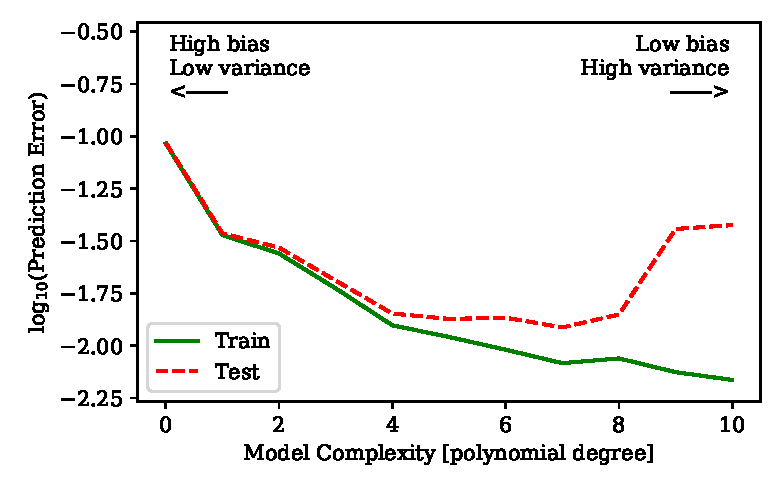
\includegraphics[scale=1]{figs/biasvariancetradeoff_ols_Franke.pdf}
    \caption{Prediction error of training and test set plotted as a function of model complexity for the OLS regression fitted on Franke's function with added noise. The data set contained 400 points.}
    \label{fig:bias_ols_Franke}
\end{figure}

\begin{figure}[H]
    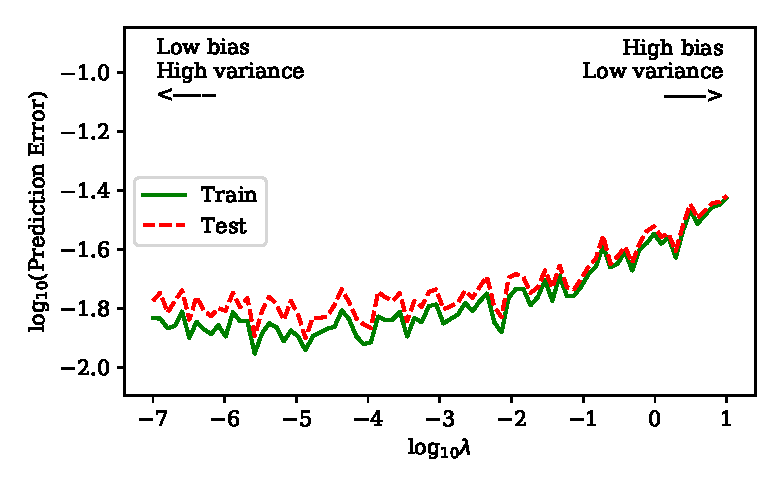
\includegraphics{figs/biasvariancetradeoff_Ridge_Franke.pdf}
    \caption{Prediction error of training and test set plotted as a function of the hyperparameter $\lambda$ for Ridge regression of degree 4 fitted on Franke's function. The total data set contained 400 points.}
    \label{fig:bias_ridge_Franke}
\end{figure}

\begin{figure}[H]
    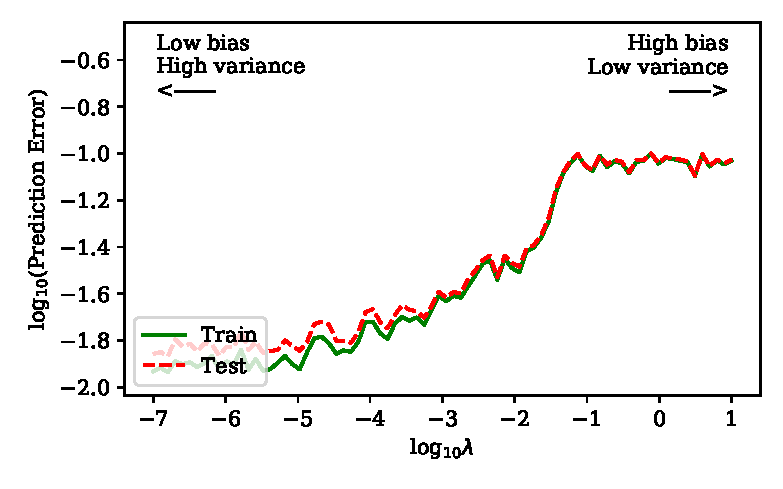
\includegraphics{figs/biasvariancetradeoff_LASSO_Franke.pdf}
    \caption{Prediction error of training and test set plotted as a function of the hyperparameter $\lambda$ for Lasso regression of degree 4 fitted on Franke's function. The total data set contained 400 points.}
    \label{fig:bias_lasso_Franke}
\end{figure}


\begin{multicols}{2}
\noindent


\begin{figure}[H]
    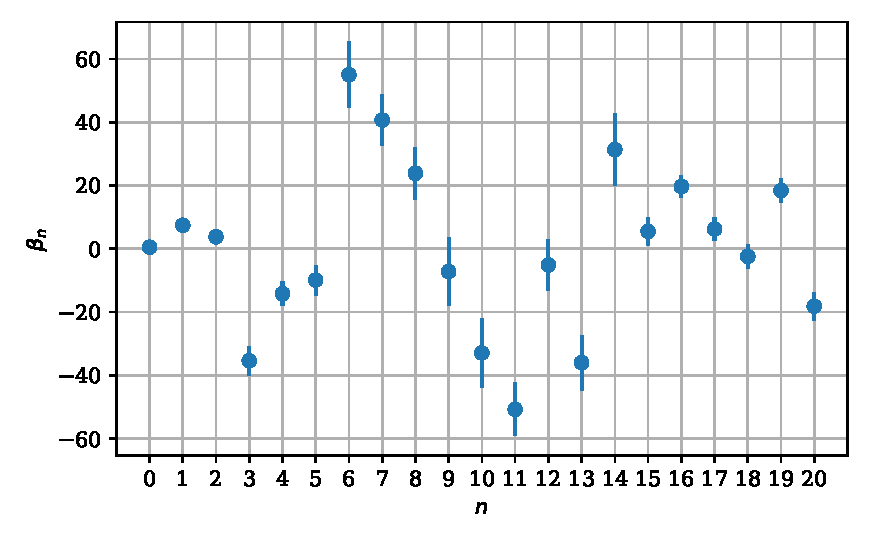
\includegraphics[scale=1]{figs/beta_variance_ols_Franke.pdf}
    \caption{OLS regression parameters $\bm{\hat{\beta}}^{\text{OLS}}_F$ of the generated Franke's function data plotted with $68\%$ confidence intervals. The total data set contained 400 points.}
    \label{fig:beta_variance_Franke}
\end{figure}
Table \ref{tab:R2} contains the $R^2$ scores for the three regression methods using a fourth order polynomial fit and $\lambda^\text{ridge}_\text{F} = \lambda^\text{lasso}_\text{F}=10^{-5}$. Looking at the EPE graphs in Figure \ref{fig:bias_ols_Franke}, \ref{fig:bias_ridge_Franke} and \ref{fig:bias_lasso_Franke}  and the $R^2$ scores, we decided that the optimal model  for the generated Franke's function data was the fourth order two-dimensional polynomial fit using OLS regression.  We have included the plot for the regression parameters $\bm{\hat{\beta}^\text{OLS}}_\text{F}$  in Figure \ref{fig:beta_variance_Franke}. To illustrate how the model fits the data, the 3D plot of the model and generated data is shown in Figure \ref{fig:3d_OLS_Franke}.

\begin{table}[H]
\caption{Table of the $R^2$ scores for both training and test sets for all three regression methods. A fourth order polynomial model was evaluated for the Franke's function data, while a tenth order polynomial was evaluated for the terrain data. \vspace{2 pt}}
\label{tab:R2}
\begin{tabular}{|c|c|c|c|} \hline
	Data set & Method & $R^2$ training & $R^2$ test\\ \hline
	\multirow{3}{*} {\makecell[l]{Franke's  \\function}}&  OLS  &  0.868 & 0.822 \\ \cline{2-4}
																		& Ridge & 0.844 &  0.819 \\ \cline{2-4}
																		& Lasso & 0.858 & 0.830 \\ \hline
	\multirow{3}{*}{Terrain} 					&  OLS  &  0.869 & 0.868 \\ \cline{2-4}
																		& Ridge & 0.868 & 0.869 \\ \cline{2-4}
																		& Lasso & 0.778 & 0.778 \\ \hline
\end{tabular}
\end{table}
\end{multicols}



\begin{figure}[H]
	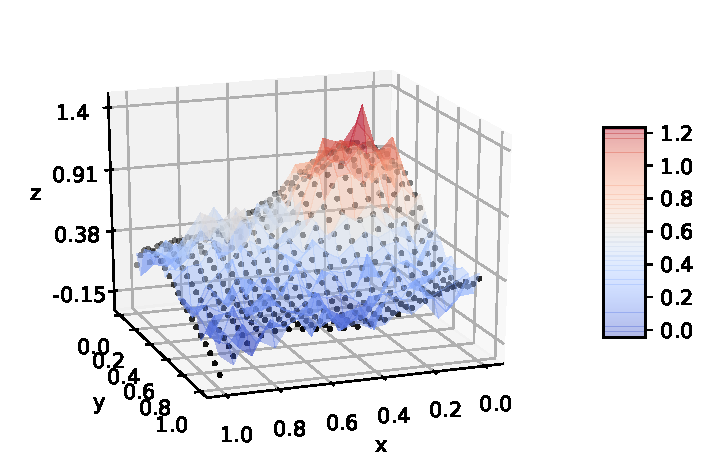
\includegraphics[scale=1]{figs/3dmodel_OLS_Franke.pdf}
	\label{fig:3d_OLS_Franke}
	\caption{3D plot of the polynomial fit with the generated Franke's function data and added noise. The fit was modeled using a fourth order two-dimensional polynomial fit with OLS regression. The total data set contained 400 points.}
\end{figure}




\subsection{Lake Tanganyika terrain data}


\begin{figure}[H]
    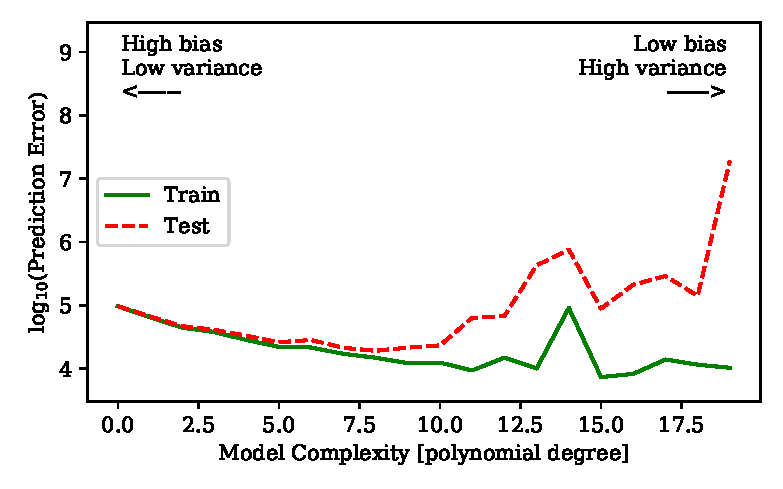
\includegraphics[scale=1]{figs/biasvariancetradeoff_ols_terrain.pdf}
    \caption{Prediction error of training and test set plotted as a function of model complexity (polynomial degree) for the ordinary least squares regression  fitted on terrain data of Lake Tanganyika, Africa. The total data set contained approximately 800 thousand points.}
    \label{fig:bias_ols_terrain}
\end{figure}

\begin{figure}[H]
    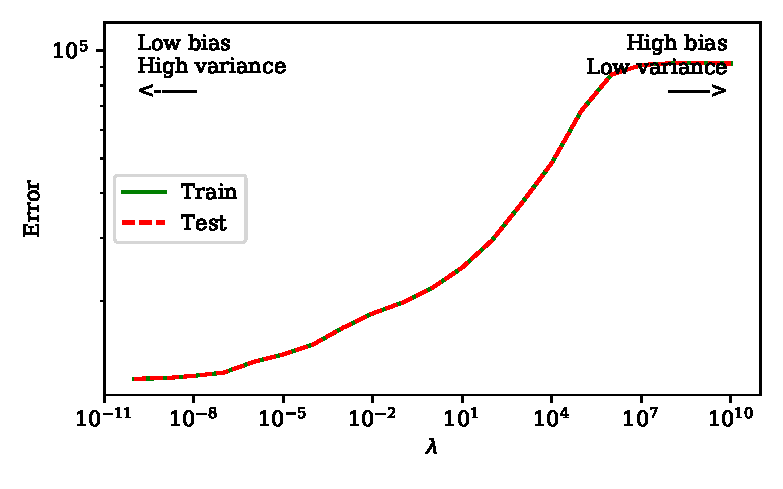
\includegraphics{figs/biasvariancetradeoff_Ridge_terrain.pdf}
    \caption{Prediction error of training and test set plotted as a function of the hyperparameter $\lambda$ for Ridge regression of degree 10 fitted on terrain data of Lake Tanganyika. The total data set contained approximately 800 thousand points.}
    \label{fig:bias_ridge_terrain}
\end{figure}

\begin{figure}[H]
    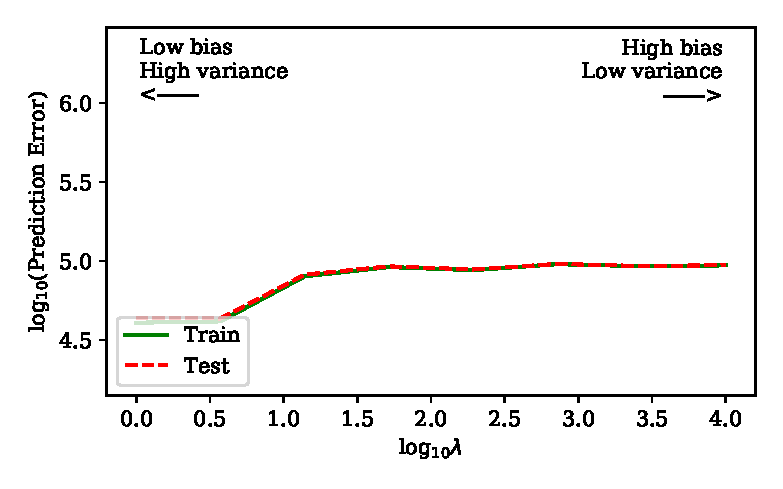
\includegraphics{figs/biasvariancetradeoff_LASSO_terrain.pdf}
    \caption{Prediction error of training and test set plotted as a function of the hyperparameter $\lambda$ for Lasso regression of degree 10 fitted on terrain data of Lake Tanganyika. The total data set contained approximately 800 thousand points.}
    \label{fig:bias_lasso_terrain}
\end{figure}

\begin{multicols}{2}
\noindent
For the Lake Tanganyika  terrain data, the EPE for the OLS regression model plotted against increasing polynomial degrees is shown in Figure \ref{fig:bias_ols_terrain}. For the terrain data we decided on using a tenth order polynomial fit for all regression methods, as the EPE for the test data seems to stabilize at degree 10 and 11, and starts increasing after.  For the shrinkage parameters, by looking at Figure \ref{fig:bias_ridge_terrain} and \ref{fig:bias_ols_terrain}, we decided on the values  $\lambda^\text{ridge}_\text{T}=10^{-10} $ and $\lambda^\text{lasso}_\text{T}=10^{-4} $.
The $R^2$ scores for the regression models  are shown in Figure \ref{tab:R2}. Considering the graphs in Figure \ref{fig:bias_ols_terrain}, \ref{fig:bias_ridge_terrain} and \ref{fig:bias_lasso_terrain} for the EPE  and the $R^2$ scores for the OLS, Ridge and Lasso regression methods, we decided that the OLS model was the best fit for our terrain.  The regression parameters $\bm{\hat{\beta}^\text{OLS}}_\text{T}$ are shown in Figure \ref{fig:beta_variance_terrain}. The 3D plot of the OLS model with the terrain data is shown in Figure \ref{fig:3d_OLS_terrain}.

\begin{figure}[H]
    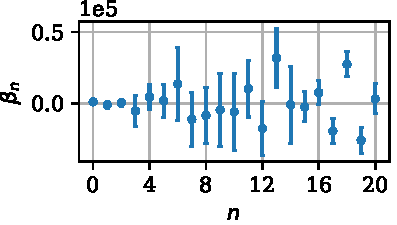
\includegraphics[scale=1]{figs/beta_variance_ols_terrain.pdf}
    \caption{OLS regression parameters $\bm{\hat{\beta}}^{\text{OLS}}_T$  of a fifth order two-dimensional polynomial model  of the terrain data from Lake Tanganyika, here plotted with $68\%$ confidence intervals. The total data set contained approximately 800 thousand points.}
    \label{fig:beta_variance_terrain}
\end{figure}

\end{multicols}

\begin{figure}[H]
	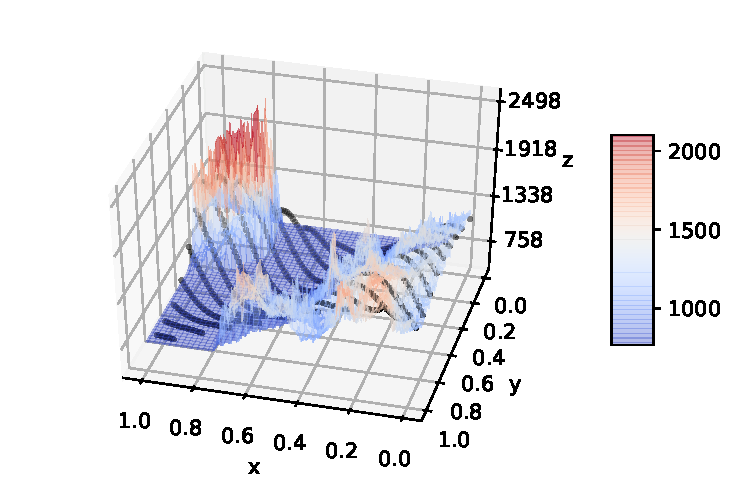
\includegraphics[scale=1]{figs/3dmodel_OLS_terrain.pdf}
	\caption{3D plot of the OLS model (dotted) and the terrain data of Lake Tanganyika. Here we have only plotted every 100th point in the $x$-direction. The total data set contained approximately 800 thousand points.}
	\label{fig:3d_OLS_terrain}

\end{figure}


\begin{multicols}{2}


\section{Discussion}
\subsection{Franke's function data}
From the $R^2$ scores for the particularly noisy ($\sigma^2 = 1$) Franke's function data in Table \ref{tab:R2_stddev=1}, it is clear that neither of the linear regression methods are sufficient for modelling this situation. The $R^2$ scores for both training and test data are quite low, with the highest training data score being 0.168 and test data score 0.105. As the variance of the noise is of the same order as Franke's function itself, the regression methods will also try to fit a polynomial to stochastic noise. This explains why the training and test set $R^2$ scores in this case correspond poorly to each other, as both contain large amounts of Gaussian noise. Due to the stochastic nature of these data, the performances of the regression methods seem to be arbitrary as well, i.e. none of the regression methods seem to be better than the others. Comparing these values to the $R^2$ scores in Table \ref{tab:R2}, where the standard deviation of the noise is $\sigma=0.1$, it seems lowering the variance was sufficient to significantly improve the $R^2$ scores of all of the polynomial fits.


Looking at Figure \ref{fig:bias_ols_Franke}, the choice of using a polynomial fit of the fourth order seems reasonable, as the test set EPE seems to stabilize at that point. From degree 4 and onwards, the difference in the training and test EPE gradually increases with  the model complexity, indicating that using a higher order fit than 4 would likely lead to overfitting of the data. However, we only used 400 data points generated using a function with added random noise, so this could likely vary for different runs of the code depending on the noise.  We are not certain if the optimal polynomial order for the OLS would be the same for the Ridge and Lasso regression, even though this was assumed in this project. Using a lower order would probably not improve the Ridge and Lasso models, but it could be interesting to examine the cases for higher orders, as the hyperparameter $\lambda$ would theoretically be able to counteract overfitting to some extent by shrinking the regression parameters.  For our results using a fourth order polynomial fit, it does seem from Figure \ref{fig:bias_ridge_Franke} and \ref{fig:bias_lasso_Franke} that the EPE is at its lowest for lower values of $\lambda_\text{F}$, suggesting that the optimal model is the OLS without any shrinkage of the parameters. It is hard to identify exactly which value of $\lambda_\text{F}$ is the optimal one within the given ranges due to the variations in these graphs. Again, using more data points would likely improve our models and smoothen the graphs.  Regardless, we are able to observe that the EPE increases sharply for higher values of $\lambda$ before plateauing in Figure \ref{fig:bias_lasso_Franke}, while the difference between the EPE for training and test data decreases. This suits our expectations of the way the hyperparameter $\lambda$ imposes a higher bias in exchange for lower variance. At the plateau, the regression parameters are shrunk to the extent that our model estimates the data as the intercept, as it is the only term exempt from the penalization. Ridge regression will force coefficients to be near-zero for sufficiently high $\lambda$, so we can thus assume the EPE for the Ridge method would behave similarly  if we increased the $\lambda$ range for which we ran cross-validation, though not as extreme as for the Lasso.

The OLS regression parameters $\bm{\hat{\beta ^\text{OLS}}}$ shown in Figure \ref{fig:beta_variance_Franke} and its  corresponding 3D plot in Figure \ref{fig:3d_OLS_Franke} seem to be the optimal model of the three. The variance of the parameters appears to be sufficiently small, and with the EPE for polynomial degree 4 being near the order of $10^{-1.8}\approx 0.016$, which seems sufficient for Franke's function, which has values of orders between  $10^{{-2}}$ and $1$.  This is not a perfect fit, which is also reflected in the $R^2$ score in Table \ref{tab:R2}, but a score of 0.822 for the test data seems satisfactory considering the simplicity of the OLS estimator. From the 3D plot, we can observe that the model is able to eliminate most of the noise from the Franke's function data, at the cost of being able to model the smaller variations in Franke's function. This is even more evident in the penalized regression methods, see our \href{https://github.com/bernharl/FYS-STK4155-project1}{Github repository} for figures, which could explain why the OLS method seems to be better for fitting this particular function. However, the $R^2$ scores for the Ridge and Lasso are still close to those of the OLS, with the Lasso test score at 0.830 surpassing that of the OLS, though this is more likely due to the variance in the data set. As the generated data only contained 400 points, the $R^2$ training scores are not identical to the test scores,  with the test score being 95 \%, 97\% and 97 \% of the training scores of OLS, Ridge and Lasso. The imposed bias in the shrinkage methods seems to produce $R^2$ test scores that are closer to the training set score for this data setz|,  although the $R^2$ training and test scores for all three methods will likely approach one another as the amount of data increases.



\subsection{Lake Tanganyika terrain data}
Figure \ref{fig:bias_ols_terrain} suggests that the optimal polynomial degree for the terrain data OLS fit lies between 10 and 11.  The EPE is almost constant within this interval, which means that opting for an 11th degree polynomial fit would not yield much better results than the tenth degree fit we chose and would also be more memory intensive. Also, for higher polynomial degrees, there seems to be what we can only assume is a numerical instability, perhaps due the inversion of a very large matrix. In theory, one would expect the training error to keep decreasing with model complexity.

The EPE graphs in Figure \ref{fig:bias_ridge_terrain} and \ref{fig:bias_lasso_terrain} show that smaller values for $\lambda$ will decrease the EPE, while higher values tend to only fit the intercept, explaining the plateau to the right in the figures. This suggests that the optimal $\lambda_\text{T}$ in this case would tend to zero. This is likely due to the fact that Ridge and Lasso are not able to model the small variations in natural terrain as well as OLS due to the shrinkage imposed by the hyperparameter. When the hyperparameter is zero, we are left with the OLS regression, which indicates that the best fit for the Lake Tanganyika terrain data is the OLS method. This is also supported by Table \ref{tab:R2}, as the highest $R^2$ scores are for the OLS and Ridge regressions at, which are nearly identical due to the choice of a very small hyperparameter $\lambda_\text{T}^\text{ridge}=10^{-10}$. The Lasso score is noticeably lower at 0.778 for both training and test data, as opposed to the 0.869 and 0.868 scores for the Ridge and OLS. Due to convergence errors, we were not able to run lower values for $\lambda_\text{T} ^\text{lasso}$, leading to our choice of $\lambda_\text{T} ^\text{lasso}=10^{-4}$. This leads to a stronger shrinkage in the Lasso fit, which causes the model to neglect the smaller variations in the terrain to a higher extent than the OLS and Ridge fits, leading to a lower $R^2$ score. Compared to for the Franke's function data, the $R^2$ training and test scores for all three fits on terrain data are nearly identical, due to the larger amount of data. The generated data set only contained 400 points, whereas the terrain data contained over 800 thousand points.  This is also apparent in the EPE graphs in Figure \ref{fig:bias_ols_terrain}, \ref{fig:bias_ridge_terrain} and \ref{fig:bias_lasso_terrain}, as the training and test graphs are overlapping completely for the terrain data, while being noticeably different for the generated data graphs in Figure \ref{fig:bias_ols_Franke}, \ref{fig:bias_ridge_Franke} and \ref{fig:bias_lasso_Franke}, particularly for higher model complexities in OLS  and smaller $\lambda$ in the Ridge and Lasso graphs.  In our \href{https://github.com/bernharl/FYS-STK4155-project1}{Github repository}, we have included corresponding figures for OLS, Ridge and Lasso on terrain data where we only used every 150th point in both directions, leading to a reduction of data points to approximately 600 points. On such a small data set, there is a visible discrepancy between the train and test errors also for the terrain data, especially in the parts of the figures where the models have low bias.

Our best terrain data fit seems to be the tenth order OLS model. Figure \ref{fig:beta_variance_terrain} shows the regression parameters $\bm{\hat{\beta}_\text{T}^\text{OLS}}$ for this model. All parameters seem to have very low variance, likely due to the amount of data used in the calculation. For comparison, we have included a figure in our \href{https://github.com/bernharl/FYS-STK4155-project1}{Github repository} where we only use about 600 data points from the terrain data, leading to much higher variance in $\bm{\hat{\beta}_\text{T}^\text{OLS}}$. 

The 3D plot of our best model is shown in Figure \ref{fig:3d_OLS_terrain}. As seen in this plot, the OLS model appears to fit the terrain data relatively well,  although it does not quite manage to model the terrain height spike surrounding the point $(1, 0)$.  There is no overfitting apparent, as the model does not seem to include any of the noise. This leads to a model that is not complex enough to model all the details, but avoids the problem of overfitting. This lack of overfitting might explain why the OLS regression performs better than the Ridge and Lasso, as penalizing should not improve the model in this case. Due to the penalty, the Lasso regression results in a worse modelling of the sharp increase in height at around $(1, 0)$, whereas Ridge, due to its small hyperparameter, is able to model this approximately peak as well as the OLS.   For the 3D plots of the Ridge and Lasso fits, see our \href{https://github.com/bernharl/FYS-STK4155-project1}{Github repository}.

Although we stated that our best fit was a tenth degree OLS model, it may also be beneficial to consider higher polynomial degrees. Higher degrees for OLS could potentially lead to overfitting, but that might not be the case for the penalized regression methods. This way we could in theory be able to better model the details of the data while also avoiding overfitting. To implement this, we could grid over various values of $\lambda_\text{T}$ and polynomial degrees for both Ridge and Lasso. A more sophisticated way could be to apply a gradient descent method to search for the minimum error as a function of $\lambda_\text{T}$ and degree. Applying either of these methods would however be far more computationally expensive than the one we used in this project. 

\section{Conclusion}
In this project, we have used three different linear regression methods on two different sets of data to examine how these regression methods work and how well they manage to model the data. The EPE and $R^2$ scores were used to evaluate the performance of the methods. The methods we used were the OLS, Ridge and Lasso on synthetic data, generated using Franke's function with added noise, and real-life terrain data from Lake Tanganyika, Africa. We used $k$-fold cross-validation with 5 folds  to find the optimal polynomial order and shrinkage parameter  for the three methods, and found that the OLS outperformed the Ridge and Lasso regression methods for both data sets using a fourth order and tenth order polynomial fit for the generated data and terrain data respectively. However, we only cross-validated different polynomial degrees for the OLS regression and assumed its optimal degree would be the same for Ridge and Lasso. We did not attempt a higher order fit in combination with different shrinkage parameters for the Ridge and Lasso regression methods, which might have yielded better fits. Nevertheless, we were able to model satisfactory fits for both data sets using OLS that were able to capture the most general trends in the data. 

\bibliographystyle{iEEEtran}
\bibliography{references}


\end{multicols}

\end{document}
